% Options for packages loaded elsewhere
\PassOptionsToPackage{unicode}{hyperref}
\PassOptionsToPackage{hyphens}{url}
\PassOptionsToPackage{dvipsnames,svgnames,x11names}{xcolor}
%
\documentclass[
  letterpaper,
  DIV=11,
  numbers=noendperiod]{scrartcl}

\usepackage{amsmath,amssymb}
\usepackage{iftex}
\ifPDFTeX
  \usepackage[T1]{fontenc}
  \usepackage[utf8]{inputenc}
  \usepackage{textcomp} % provide euro and other symbols
\else % if luatex or xetex
  \usepackage{unicode-math}
  \defaultfontfeatures{Scale=MatchLowercase}
  \defaultfontfeatures[\rmfamily]{Ligatures=TeX,Scale=1}
\fi
\usepackage{lmodern}
\ifPDFTeX\else  
    % xetex/luatex font selection
\fi
% Use upquote if available, for straight quotes in verbatim environments
\IfFileExists{upquote.sty}{\usepackage{upquote}}{}
\IfFileExists{microtype.sty}{% use microtype if available
  \usepackage[]{microtype}
  \UseMicrotypeSet[protrusion]{basicmath} % disable protrusion for tt fonts
}{}
\makeatletter
\@ifundefined{KOMAClassName}{% if non-KOMA class
  \IfFileExists{parskip.sty}{%
    \usepackage{parskip}
  }{% else
    \setlength{\parindent}{0pt}
    \setlength{\parskip}{6pt plus 2pt minus 1pt}}
}{% if KOMA class
  \KOMAoptions{parskip=half}}
\makeatother
\usepackage{xcolor}
\setlength{\emergencystretch}{3em} % prevent overfull lines
\setcounter{secnumdepth}{-\maxdimen} % remove section numbering
% Make \paragraph and \subparagraph free-standing
\makeatletter
\ifx\paragraph\undefined\else
  \let\oldparagraph\paragraph
  \renewcommand{\paragraph}{
    \@ifstar
      \xxxParagraphStar
      \xxxParagraphNoStar
  }
  \newcommand{\xxxParagraphStar}[1]{\oldparagraph*{#1}\mbox{}}
  \newcommand{\xxxParagraphNoStar}[1]{\oldparagraph{#1}\mbox{}}
\fi
\ifx\subparagraph\undefined\else
  \let\oldsubparagraph\subparagraph
  \renewcommand{\subparagraph}{
    \@ifstar
      \xxxSubParagraphStar
      \xxxSubParagraphNoStar
  }
  \newcommand{\xxxSubParagraphStar}[1]{\oldsubparagraph*{#1}\mbox{}}
  \newcommand{\xxxSubParagraphNoStar}[1]{\oldsubparagraph{#1}\mbox{}}
\fi
\makeatother

\usepackage{color}
\usepackage{fancyvrb}
\newcommand{\VerbBar}{|}
\newcommand{\VERB}{\Verb[commandchars=\\\{\}]}
\DefineVerbatimEnvironment{Highlighting}{Verbatim}{commandchars=\\\{\}}
% Add ',fontsize=\small' for more characters per line
\usepackage{framed}
\definecolor{shadecolor}{RGB}{241,243,245}
\newenvironment{Shaded}{\begin{snugshade}}{\end{snugshade}}
\newcommand{\AlertTok}[1]{\textcolor[rgb]{0.68,0.00,0.00}{#1}}
\newcommand{\AnnotationTok}[1]{\textcolor[rgb]{0.37,0.37,0.37}{#1}}
\newcommand{\AttributeTok}[1]{\textcolor[rgb]{0.40,0.45,0.13}{#1}}
\newcommand{\BaseNTok}[1]{\textcolor[rgb]{0.68,0.00,0.00}{#1}}
\newcommand{\BuiltInTok}[1]{\textcolor[rgb]{0.00,0.23,0.31}{#1}}
\newcommand{\CharTok}[1]{\textcolor[rgb]{0.13,0.47,0.30}{#1}}
\newcommand{\CommentTok}[1]{\textcolor[rgb]{0.37,0.37,0.37}{#1}}
\newcommand{\CommentVarTok}[1]{\textcolor[rgb]{0.37,0.37,0.37}{\textit{#1}}}
\newcommand{\ConstantTok}[1]{\textcolor[rgb]{0.56,0.35,0.01}{#1}}
\newcommand{\ControlFlowTok}[1]{\textcolor[rgb]{0.00,0.23,0.31}{\textbf{#1}}}
\newcommand{\DataTypeTok}[1]{\textcolor[rgb]{0.68,0.00,0.00}{#1}}
\newcommand{\DecValTok}[1]{\textcolor[rgb]{0.68,0.00,0.00}{#1}}
\newcommand{\DocumentationTok}[1]{\textcolor[rgb]{0.37,0.37,0.37}{\textit{#1}}}
\newcommand{\ErrorTok}[1]{\textcolor[rgb]{0.68,0.00,0.00}{#1}}
\newcommand{\ExtensionTok}[1]{\textcolor[rgb]{0.00,0.23,0.31}{#1}}
\newcommand{\FloatTok}[1]{\textcolor[rgb]{0.68,0.00,0.00}{#1}}
\newcommand{\FunctionTok}[1]{\textcolor[rgb]{0.28,0.35,0.67}{#1}}
\newcommand{\ImportTok}[1]{\textcolor[rgb]{0.00,0.46,0.62}{#1}}
\newcommand{\InformationTok}[1]{\textcolor[rgb]{0.37,0.37,0.37}{#1}}
\newcommand{\KeywordTok}[1]{\textcolor[rgb]{0.00,0.23,0.31}{\textbf{#1}}}
\newcommand{\NormalTok}[1]{\textcolor[rgb]{0.00,0.23,0.31}{#1}}
\newcommand{\OperatorTok}[1]{\textcolor[rgb]{0.37,0.37,0.37}{#1}}
\newcommand{\OtherTok}[1]{\textcolor[rgb]{0.00,0.23,0.31}{#1}}
\newcommand{\PreprocessorTok}[1]{\textcolor[rgb]{0.68,0.00,0.00}{#1}}
\newcommand{\RegionMarkerTok}[1]{\textcolor[rgb]{0.00,0.23,0.31}{#1}}
\newcommand{\SpecialCharTok}[1]{\textcolor[rgb]{0.37,0.37,0.37}{#1}}
\newcommand{\SpecialStringTok}[1]{\textcolor[rgb]{0.13,0.47,0.30}{#1}}
\newcommand{\StringTok}[1]{\textcolor[rgb]{0.13,0.47,0.30}{#1}}
\newcommand{\VariableTok}[1]{\textcolor[rgb]{0.07,0.07,0.07}{#1}}
\newcommand{\VerbatimStringTok}[1]{\textcolor[rgb]{0.13,0.47,0.30}{#1}}
\newcommand{\WarningTok}[1]{\textcolor[rgb]{0.37,0.37,0.37}{\textit{#1}}}

\providecommand{\tightlist}{%
  \setlength{\itemsep}{0pt}\setlength{\parskip}{0pt}}\usepackage{longtable,booktabs,array}
\usepackage{calc} % for calculating minipage widths
% Correct order of tables after \paragraph or \subparagraph
\usepackage{etoolbox}
\makeatletter
\patchcmd\longtable{\par}{\if@noskipsec\mbox{}\fi\par}{}{}
\makeatother
% Allow footnotes in longtable head/foot
\IfFileExists{footnotehyper.sty}{\usepackage{footnotehyper}}{\usepackage{footnote}}
\makesavenoteenv{longtable}
\usepackage{graphicx}
\makeatletter
\def\maxwidth{\ifdim\Gin@nat@width>\linewidth\linewidth\else\Gin@nat@width\fi}
\def\maxheight{\ifdim\Gin@nat@height>\textheight\textheight\else\Gin@nat@height\fi}
\makeatother
% Scale images if necessary, so that they will not overflow the page
% margins by default, and it is still possible to overwrite the defaults
% using explicit options in \includegraphics[width, height, ...]{}
\setkeys{Gin}{width=\maxwidth,height=\maxheight,keepaspectratio}
% Set default figure placement to htbp
\makeatletter
\def\fps@figure{htbp}
\makeatother

\KOMAoption{captions}{tableheading}
\makeatletter
\@ifpackageloaded{caption}{}{\usepackage{caption}}
\AtBeginDocument{%
\ifdefined\contentsname
  \renewcommand*\contentsname{Table of contents}
\else
  \newcommand\contentsname{Table of contents}
\fi
\ifdefined\listfigurename
  \renewcommand*\listfigurename{List of Figures}
\else
  \newcommand\listfigurename{List of Figures}
\fi
\ifdefined\listtablename
  \renewcommand*\listtablename{List of Tables}
\else
  \newcommand\listtablename{List of Tables}
\fi
\ifdefined\figurename
  \renewcommand*\figurename{Figure}
\else
  \newcommand\figurename{Figure}
\fi
\ifdefined\tablename
  \renewcommand*\tablename{Table}
\else
  \newcommand\tablename{Table}
\fi
}
\@ifpackageloaded{float}{}{\usepackage{float}}
\floatstyle{ruled}
\@ifundefined{c@chapter}{\newfloat{codelisting}{h}{lop}}{\newfloat{codelisting}{h}{lop}[chapter]}
\floatname{codelisting}{Listing}
\newcommand*\listoflistings{\listof{codelisting}{List of Listings}}
\makeatother
\makeatletter
\makeatother
\makeatletter
\@ifpackageloaded{caption}{}{\usepackage{caption}}
\@ifpackageloaded{subcaption}{}{\usepackage{subcaption}}
\makeatother

\ifLuaTeX
  \usepackage{selnolig}  % disable illegal ligatures
\fi
\usepackage{bookmark}

\IfFileExists{xurl.sty}{\usepackage{xurl}}{} % add URL line breaks if available
\urlstyle{same} % disable monospaced font for URLs
\hypersetup{
  pdftitle={Rapport technique - CC STA205 - Erwan Louveau, Louis Cazade, Alarig Vigneras},
  colorlinks=true,
  linkcolor={blue},
  filecolor={Maroon},
  citecolor={Blue},
  urlcolor={Blue},
  pdfcreator={LaTeX via pandoc}}


\title{Rapport technique - CC STA205 - Erwan Louveau, Louis Cazade,
Alarig Vigneras}
\author{}
\date{}

\begin{document}
\maketitle


\begin{verbatim}
Warning: le package 'survminer' a été compilé avec la version R 4.4.2
\end{verbatim}

\begin{verbatim}
Le chargement a nécessité le package : ggplot2
\end{verbatim}

\begin{verbatim}
Le chargement a nécessité le package : ggpubr
\end{verbatim}

\begin{verbatim}
Warning: le package 'ggpubr' a été compilé avec la version R 4.4.2
\end{verbatim}

\begin{verbatim}

Attachement du package : 'survminer'
\end{verbatim}

\begin{verbatim}
L'objet suivant est masqué depuis 'package:survival':

    myeloma
\end{verbatim}

\begin{verbatim}

Attachement du package : 'dplyr'
\end{verbatim}

\begin{verbatim}
Les objets suivants sont masqués depuis 'package:stats':

    filter, lag
\end{verbatim}

\begin{verbatim}
Les objets suivants sont masqués depuis 'package:base':

    intersect, setdiff, setequal, union
\end{verbatim}

\begin{verbatim}

-- Column specification --------------------------------------------------------
cols(
  ID = col_double(),
  Age = col_double(),
  Sodium = col_double(),
  dc = col_double(),
  temps = col_double(),
  sexe = col_double(),
  tabac = col_double(),
  hta = col_double(),
  diabete = col_double(),
  anemie = col_double(),
  fraction = col_double(),
  creat = col_double(),
  creatk = col_double()
)
\end{verbatim}

\subsection{Estimation de la fonction de survie -
Kaplan-Meier}\label{estimation-de-la-fonction-de-survie---kaplan-meier}

\begin{Shaded}
\begin{Highlighting}[]
\NormalTok{fit }\OtherTok{\textless{}{-}} \FunctionTok{survfit}\NormalTok{(}\FunctionTok{Surv}\NormalTok{(temps,dc}\SpecialCharTok{==}\DecValTok{1}\NormalTok{) }\SpecialCharTok{\textasciitilde{}}\NormalTok{ fractionF, }\AttributeTok{data =}\NormalTok{ data)}
\FunctionTok{ggsurvplot}\NormalTok{(}
\NormalTok{  fit, }
  \AttributeTok{data =}\NormalTok{ data,}
  \AttributeTok{conf.int =} \ConstantTok{TRUE}\NormalTok{,}
  \AttributeTok{pval =} \ConstantTok{FALSE}\NormalTok{,}
  \AttributeTok{risk.table =} \ConstantTok{FALSE}\NormalTok{,}
  \AttributeTok{ggtheme =} \FunctionTok{theme\_minimal}\NormalTok{()}
\NormalTok{)}
\end{Highlighting}
\end{Shaded}

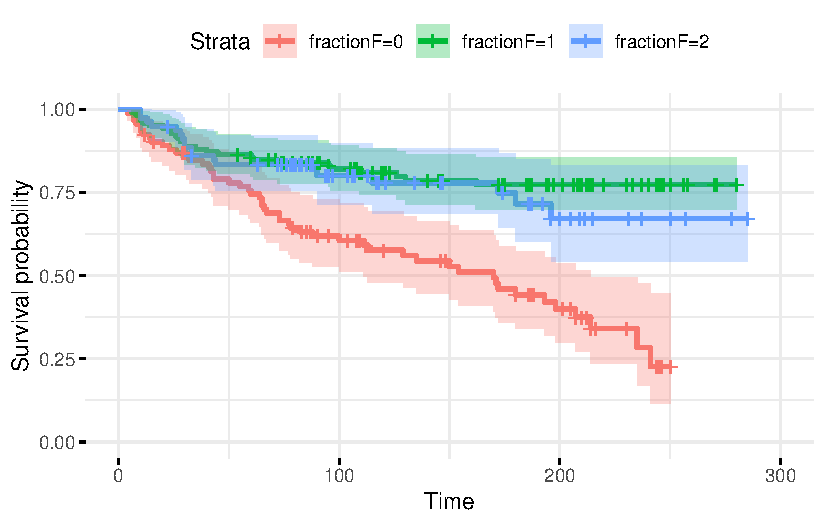
\includegraphics{Rapport-technique_files/figure-pdf/unnamed-chunk-2-1.pdf}

\subsection{Modèle sans interaction ni
stratification}\label{moduxe8le-sans-interaction-ni-stratification}

\begin{Shaded}
\begin{Highlighting}[]
\NormalTok{fit }\OtherTok{\textless{}{-}} \FunctionTok{coxph}\NormalTok{(}\FunctionTok{Surv}\NormalTok{(temps, dc }\SpecialCharTok{==} \DecValTok{1}\NormalTok{) }\SpecialCharTok{\textasciitilde{}}\NormalTok{ fractionF }\SpecialCharTok{+}\NormalTok{ sexe }\SpecialCharTok{+}\NormalTok{ AgeC }\SpecialCharTok{+}\NormalTok{ tabac }\SpecialCharTok{+}\NormalTok{ hta }\SpecialCharTok{+}\NormalTok{ diabete }\SpecialCharTok{+}\NormalTok{ Sodium }\SpecialCharTok{+}\NormalTok{ anemie }\SpecialCharTok{+}\NormalTok{ insufisanceR }\SpecialCharTok{+}\NormalTok{ creatk, }
             \AttributeTok{data =}\NormalTok{ data, }\AttributeTok{ties =} \StringTok{\textquotesingle{}breslow\textquotesingle{}}\NormalTok{)}
\FunctionTok{summary}\NormalTok{(fit)}
\end{Highlighting}
\end{Shaded}

\begin{verbatim}
Call:
coxph(formula = Surv(temps, dc == 1) ~ fractionF + sexe + AgeC + 
    tabac + hta + diabete + Sodium + anemie + insufisanceR + 
    creatk, data = data, ties = "breslow")

  n= 299, number of events= 96 

                    coef  exp(coef)   se(coef)      z Pr(>|z|)    
fractionF1    -1.092e+00  3.357e-01  2.625e-01 -4.159 3.20e-05 ***
fractionF2    -7.552e-01  4.699e-01  2.867e-01 -2.634 0.008431 ** 
sexe2          1.911e-01  1.211e+00  2.395e-01  0.798 0.424754    
AgeC           4.825e-02  1.049e+00  9.442e-03  5.110 3.22e-07 ***
tabac1         1.305e-01  1.139e+00  2.451e-01  0.532 0.594393    
hta1           5.074e-01  1.661e+00  2.163e-01  2.345 0.019003 *  
diabete1       2.156e-01  1.241e+00  2.267e-01  0.951 0.341625    
Sodium        -4.414e-02  9.568e-01  2.271e-02 -1.944 0.051945 .  
anemie1        3.791e-01  1.461e+00  2.200e-01  1.723 0.084848 .  
insufisanceR1  8.251e-01  2.282e+00  2.375e-01  3.475 0.000512 ***
creatk         2.828e-04  1.000e+00  9.952e-05  2.842 0.004488 ** 
---
Signif. codes:  0 '***' 0.001 '**' 0.01 '*' 0.05 '.' 0.1 ' ' 1

              exp(coef) exp(-coef) lower .95 upper .95
fractionF1       0.3357     2.9790    0.2007    0.5615
fractionF2       0.4699     2.1279    0.2679    0.8242
sexe2            1.2106     0.8260    0.7571    1.9358
AgeC             1.0494     0.9529    1.0302    1.0690
tabac1           1.1394     0.8776    0.7047    1.8423
hta1             1.6609     0.6021    1.0870    2.5379
diabete1         1.2406     0.8060    0.7955    1.9348
Sodium           0.9568     1.0451    0.9152    1.0004
anemie1          1.4609     0.6845    0.9493    2.2484
insufisanceR1    2.2822     0.4382    1.4329    3.6349
creatk           1.0003     0.9997    1.0001    1.0005

Concordance= 0.746  (se = 0.025 )
Likelihood ratio test= 87.55  on 11 df,   p=5e-14
Wald test            = 86.27  on 11 df,   p=9e-14
Score (logrank) test = 93.47  on 11 df,   p=3e-15
\end{verbatim}

\subsection{Modèle avec interaction et
stratification}\label{moduxe8le-avec-interaction-et-stratification}

\begin{Shaded}
\begin{Highlighting}[]
\NormalTok{fitf }\OtherTok{\textless{}{-}} \FunctionTok{coxph}\NormalTok{(}\FunctionTok{Surv}\NormalTok{(temps, dc }\SpecialCharTok{==} \DecValTok{1}\NormalTok{) }\SpecialCharTok{\textasciitilde{}}\NormalTok{ fractionF }\SpecialCharTok{+}\NormalTok{ sexe }\SpecialCharTok{+}\NormalTok{ AgeC }\SpecialCharTok{+}\NormalTok{ tabac }\SpecialCharTok{+}\NormalTok{ hta }\SpecialCharTok{+}\NormalTok{ diabete }\SpecialCharTok{+}\NormalTok{ Sodium }\SpecialCharTok{+}\NormalTok{ anemie }\SpecialCharTok{+}\NormalTok{ creatk }\SpecialCharTok{+} \FunctionTok{strata}\NormalTok{(insufisanceR) }\SpecialCharTok{+} \FunctionTok{tt}\NormalTok{(}\FunctionTok{as.numeric}\NormalTok{(fractionF)) }\SpecialCharTok{+}\NormalTok{ diabete}\SpecialCharTok{*}\NormalTok{Sodium }\SpecialCharTok{+}\NormalTok{ tabac}\SpecialCharTok{*}\NormalTok{sexe, }
              \AttributeTok{data =}\NormalTok{ data, }\AttributeTok{ties =} \StringTok{\textquotesingle{}breslow\textquotesingle{}}\NormalTok{, }\AttributeTok{tt=}\ControlFlowTok{function}\NormalTok{(x, t, ...)\{x }\SpecialCharTok{*}\NormalTok{ t\})}
\FunctionTok{summary}\NormalTok{(fitf)}
\end{Highlighting}
\end{Shaded}

\begin{verbatim}
Call:
coxph(formula = Surv(temps, dc == 1) ~ fractionF + sexe + AgeC + 
    tabac + hta + diabete + Sodium + anemie + creatk + strata(insufisanceR) + 
    tt(as.numeric(fractionF)) + diabete * Sodium + tabac * sexe, 
    data = data, ties = "breslow", tt = function(x, t, ...) {
        x * t
    })

  n= 299, number of events= 96 

                                coef  exp(coef)   se(coef)      z Pr(>|z|)    
fractionF1                -7.791e-01  4.588e-01  3.285e-01 -2.372  0.01770 *  
fractionF2                -3.140e-01  7.305e-01  4.191e-01 -0.749  0.45362    
sexe2                      1.285e-01  1.137e+00  2.570e-01  0.500  0.61726    
AgeC                       4.914e-02  1.050e+00  9.783e-03  5.022 5.11e-07 ***
tabac1                     5.165e-02  1.053e+00  2.686e-01  0.192  0.84752    
hta1                       5.256e-01  1.691e+00  2.226e-01  2.361  0.01824 *  
diabete1                  -5.171e+00  5.680e-03  6.471e+00 -0.799  0.42424    
Sodium                    -6.538e-02  9.367e-01  3.886e-02 -1.683  0.09245 .  
anemie1                    4.417e-01  1.555e+00  2.278e-01  1.939  0.05252 .  
creatk                     2.802e-04  1.000e+00  9.695e-05  2.890  0.00385 ** 
tt(as.numeric(fractionF)) -3.281e-03  9.967e-01  2.671e-03 -1.228  0.21929    
diabete1:Sodium            3.991e-02  1.041e+00  4.769e-02  0.837  0.40265    
sexe2:tabac1               5.050e-01  1.657e+00  7.068e-01  0.715  0.47489    
---
Signif. codes:  0 '***' 0.001 '**' 0.01 '*' 0.05 '.' 0.1 ' ' 1

                          exp(coef) exp(-coef) lower .95 upper .95
fractionF1                  0.45882     2.1795 2.410e-01    0.8734
fractionF2                  0.73048     1.3690 3.213e-01    1.6608
sexe2                       1.13707     0.8795 6.871e-01    1.8818
AgeC                        1.05036     0.9521 1.030e+00    1.0707
tabac1                      1.05301     0.9497 6.220e-01    1.7827
hta1                        1.69144     0.5912 1.093e+00    2.6168
diabete1                    0.00568   176.0458 1.764e-08 1829.4957
Sodium                      0.93671     1.0676 8.680e-01    1.0108
anemie1                     1.55537     0.6429 9.952e-01    2.4308
creatk                      1.00028     0.9997 1.000e+00    1.0005
tt(as.numeric(fractionF))   0.99672     1.0033 9.915e-01    1.0020
diabete1:Sodium             1.04072     0.9609 9.479e-01    1.1427
sexe2:tabac1                1.65705     0.6035 4.147e-01    6.6215

Concordance= 0.732  (se = 0.029 )
Likelihood ratio test= 59.97  on 13 df,   p=5e-08
Wald test            = 56.49  on 13 df,   p=2e-07
Score (logrank) test = 59.78  on 13 df,   p=6e-08
\end{verbatim}

\subsection{Résidus de Schoenfeld}\label{ruxe9sidus-de-schoenfeld}

\begin{Shaded}
\begin{Highlighting}[]
\NormalTok{prop1 }\OtherTok{\textless{}{-}} \FunctionTok{cox.zph}\NormalTok{(fit,}\AttributeTok{transform=}\StringTok{"identity"}\NormalTok{)}
\FunctionTok{print}\NormalTok{(prop1)}
\end{Highlighting}
\end{Shaded}

\begin{verbatim}
                chisq df      p
fractionF    9.56e+00  2 0.0084
sexe         3.23e-02  1 0.8573
AgeC         3.48e-04  1 0.9851
tabac        1.46e+00  1 0.2277
hta          2.78e-01  1 0.5983
diabete      5.25e-01  1 0.4685
Sodium       4.59e-02  1 0.8304
anemie       2.10e-02  1 0.8848
insufisanceR 5.24e+00  1 0.0221
creatk       1.31e+00  1 0.2529
GLOBAL       2.01e+01 11 0.0438
\end{verbatim}

\begin{Shaded}
\begin{Highlighting}[]
\FunctionTok{plot}\NormalTok{(prop1[}\DecValTok{1}\NormalTok{]) }\CommentTok{\# résidus de schoenfeld de la variable fraction d\textquotesingle{}éjection}
\end{Highlighting}
\end{Shaded}

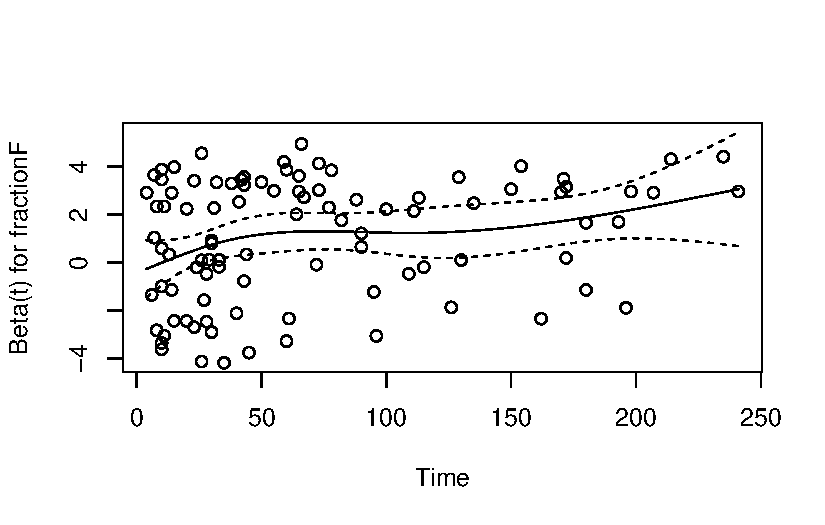
\includegraphics{Rapport-technique_files/figure-pdf/unnamed-chunk-5-1.pdf}

\begin{Shaded}
\begin{Highlighting}[]
\FunctionTok{plot}\NormalTok{(prop1[}\DecValTok{9}\NormalTok{]) }\CommentTok{\# résidus de schoenfeld de la variable insuffisance rénale}
\end{Highlighting}
\end{Shaded}

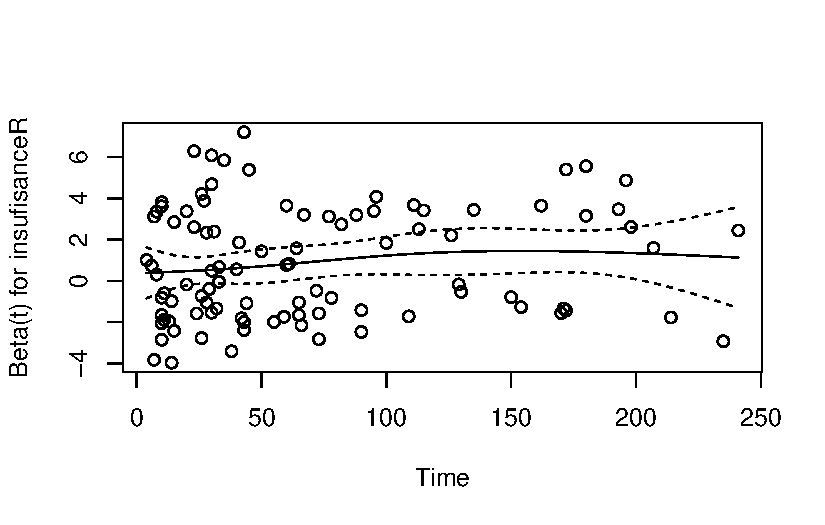
\includegraphics{Rapport-technique_files/figure-pdf/unnamed-chunk-5-2.pdf}

\subsection{Résidus de martingale du modèle sans interaction ni
stratification}\label{ruxe9sidus-de-martingale-du-moduxe8le-sans-interaction-ni-stratification}

\begin{Shaded}
\begin{Highlighting}[]
\FunctionTok{plot}\NormalTok{(}\FunctionTok{predict}\NormalTok{(fit), }\FunctionTok{residuals}\NormalTok{(fit,}\AttributeTok{type =} \StringTok{"martingale"}\NormalTok{),}
     \AttributeTok{xlab =} \StringTok{"fitted value"}\NormalTok{, }\AttributeTok{ylab =} \StringTok{"Martingale Residuals"}\NormalTok{, }\AttributeTok{las =} \DecValTok{1}\NormalTok{)}
\FunctionTok{abline}\NormalTok{(}\AttributeTok{h=}\DecValTok{0}\NormalTok{, }\AttributeTok{col=}\StringTok{"red"}\NormalTok{)}
\end{Highlighting}
\end{Shaded}

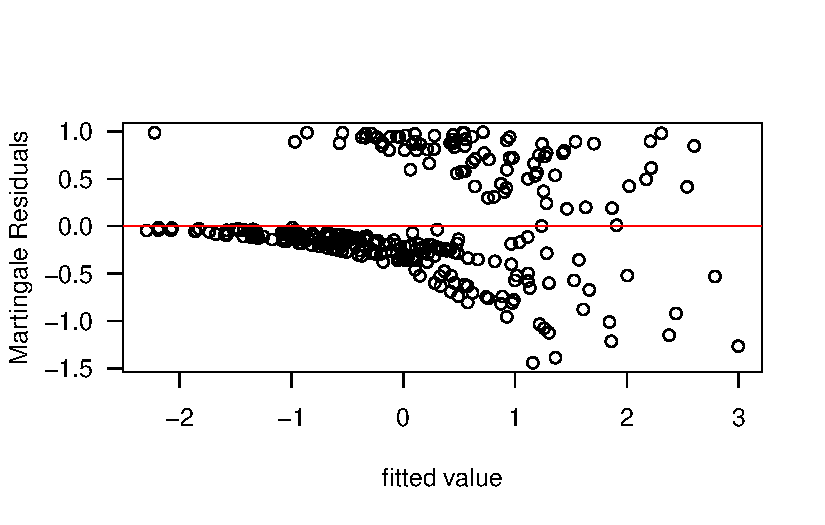
\includegraphics{Rapport-technique_files/figure-pdf/unnamed-chunk-6-1.pdf}

\subsection{Résidus de martingale du modèle avec interaction et
stratification}\label{ruxe9sidus-de-martingale-du-moduxe8le-avec-interaction-et-stratification}

\begin{Shaded}
\begin{Highlighting}[]
\FunctionTok{plot}\NormalTok{(}\FunctionTok{predict}\NormalTok{(fitf), }\FunctionTok{residuals}\NormalTok{(fitf,}\AttributeTok{type =} \StringTok{"martingale"}\NormalTok{),}
     \AttributeTok{xlab =} \StringTok{"fitted value"}\NormalTok{, }\AttributeTok{ylab =} \StringTok{"Martingale Residuals"}\NormalTok{, }\AttributeTok{las =} \DecValTok{1}\NormalTok{)}
\FunctionTok{abline}\NormalTok{(}\AttributeTok{h=}\DecValTok{0}\NormalTok{, }\AttributeTok{col =}\StringTok{"red"}\NormalTok{)}
\end{Highlighting}
\end{Shaded}

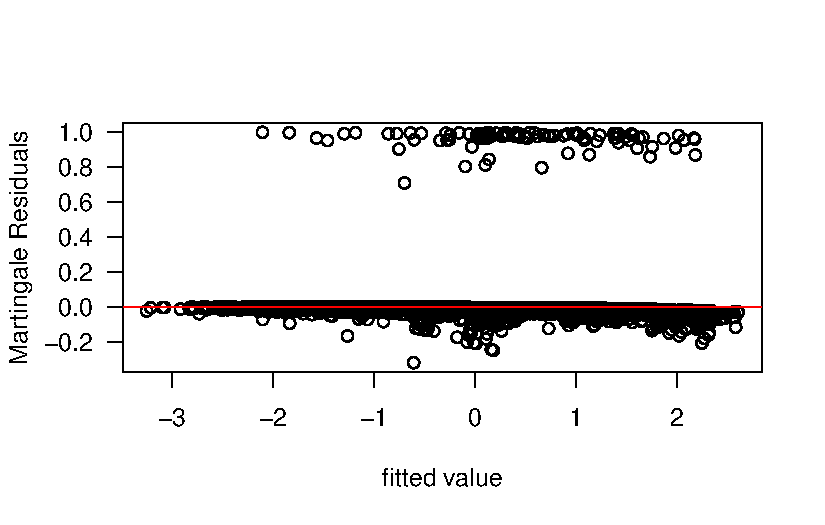
\includegraphics{Rapport-technique_files/figure-pdf/unnamed-chunk-7-1.pdf}




\end{document}
